Om met native ontwikkeling van start te gaan, wordt Android Studio eerst gedownload. 

\paragraph{1. Components}
Bij het eerste scherm van het installatieprogramma is het belangrijk om ook 
\textbf{Android Virtual Device} te selecteren. Dit is de emulator die gebruikt 
zal worden om de applicaties te runnen.

\paragraph{2. Installatie locatie}
Op het volgende scherm wordt de locatie waar Android Studio geïnstalleerd wordt gekozen. 
Het is aan te raden om dit niet te vervangen omdat React Native gebruik maakt van de standaard 
locatie om bepaalde componenten op te zoeken. 

\paragraph{3. Startmenu map}
Deze is zelf te kiezen. Hiermee wordt een shortcut gecreëerd vanwaar Android Studio kan worden opgestart.

\paragraph{4. Android SDK}\label{par:sdk}
Als de installatie goed is verlopen, wordt volgend scherm getoond. 
\begin{figure}[H]
    \centering
    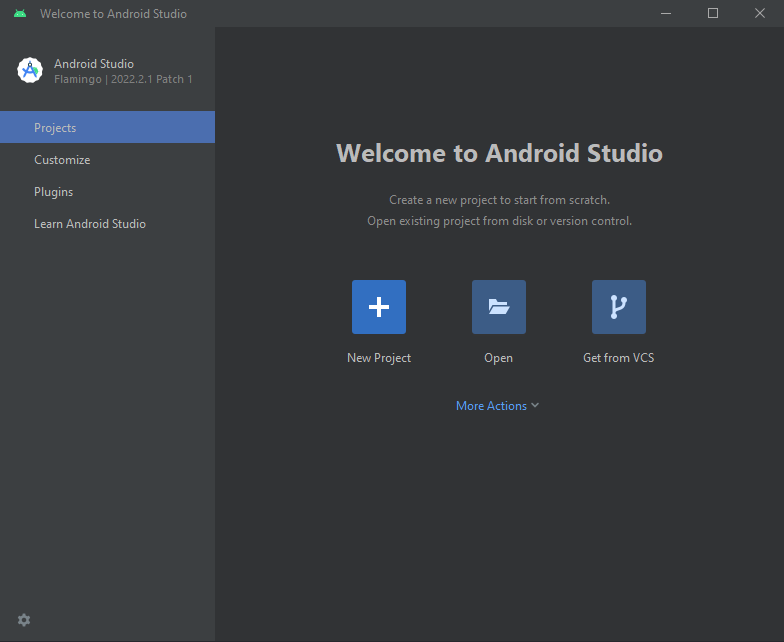
\includegraphics[height=0.4\textheight]{androidinstallatie.png}
    \caption{Startscherm na Android Studio installatie.}
\end{figure}
Standaard wordt de laatste Android SDK geïnstalleerd door Android Studio. 
Deze wordt ook tijdens de duur van het onderzoek gebruikt. 
Om met deze laatste Android SDK te werken, is Android 13 (Tiramisu) nodig. 
Deze wordt geïnstalleerd door op \textit{More Actions} te drukken. Op het nieuwe verkregen scherm 
kan Android 13 (Tiramisu) dan worden aangevinkt. Ook moet onderaan rechts het vakje 
\textbf{Show Package Details} aangevinkt worden, om dan te verifiëren dat de 
\textbf{Android SDK Platform 33}, \textbf{Sources for Android 33} en 
\textbf{Google APIs Intel x86\_64 Atom System Image} zijn aangevinkt.
\\\\
Daarna wordt er genavigeerd naar SDK Tools en wordt \textbf{Show Package Details} 
en \textbf{33.0.0} onder Android SDK Build-Tools aangevinkt. 
Tot slot wordt er op \textbf{Apply} gedrukt om de Android SDK en gerelateerde tools te downloaden en installeren.
Daarna kan een dummy project worden aangemaakt (Empty Activity) om Android Studio van start te krijgen.

\paragraph{5. Emulator}
Om de applicaties die doorheen het onderzoek ontwikkeld worden te runnen, is een emulator nodig. 
Deze wordt aangemaakt bovenaan rechts \textit{Device Manager > Create device}. 
Eerst en vooral wordt de device geselecteerd die gesimuleerd wordt. Voor het onderzoek 
wordt een Pixel 3 als emulator gebruikt. Na het selecteren van de device wordt de Android versie gekozen. 
Hier wordt Tiramisu met API Level 33 (die daarnet is geïnstalleerd) geselecteerd. 
Tot slot zijn er nog een aantal configuratie instellingen voor het apparaat. Voor het onderzoek worden 
de standaard instellingen gebruikt.
\\\\
Nu is Android Studio klaar om native applicaties te ontwikkelen en runnen. 
